\documentclass[journal,12pt,twocolumn]{IEEEtran}

\usepackage{enumitem}
\usepackage{amsmath}
\usepackage{amssymb}
\usepackage{gensymb}
\usepackage{graphicx}
\usepackage{txfonts}         
\usepackage{listings}
\usepackage{lstautogobble}
\usepackage{mathtools}
\providecommand{\dec}[2]{\ensuremath{\overset{#1}{\underset{#2}{\gtrless}}}}
	\newcommand{\myvec}[1]{\ensuremath{\begin{pmatrix}#1\end{pmatrix}}}
	\newcommand{\mydet}[1]{\ensuremath{\begin{vmatrix}#1\end{vmatrix}}}
\newcommand{\solution}{\noindent \textbf{Solution: }}
\providecommand{\pr}[1]{\ensuremath{\Pr\left(#1\right)}}
\providecommand{\brak}[1]{\ensuremath{\left(#1\right)}}
\providecommand{\cbrak}[1]{\ensuremath{\left\{#1\right\}}}
\providecommand{\sbrak}[1]{\ensuremath{\left[#1\right]}}
\providecommand{\mean}[1]{E\left[ #1 \right]}
\providecommand{\var}[1]{\mathrm{Var}\left[ #1 \right]}
\providecommand{\der}[1]{\mathrm{d} #1}

\let\StandardTheFigure\thefigure
\numberwithin{equation}{section}
\renewcommand{\thefigure}{\theenumi}
\renewcommand\thesection{\arabic{section}}

\lstset {
	frame=single, 
	breaklines=true,
	columns=fullflexible,
	autogobble=true
}             
                               
\title{Random Numbers }
\author{Ravula Karthik \\ \normalsize AI21BTECH11024 \\ \vspace*{20pt} \normalsize }


\begin{document}

	\maketitle
	
	\section{Uniform Random Numbers}
	Let $U$ be a uniform random variable between 0 and 1.
	\begin{enumerate}[label=\thesection.\arabic*,ref=\thesection.\theenumi]
	\item Generate $10^6$ samples of $U$ using a C program and save into a file called uni.dat

	\solution The c code for 1.1 can be obtained from
	\begin{lstlisting}
		wget https://github.com/karthik6281/AI1110-Assignments/blob/main/random_numbers/1/exrand.c
		wget https://github.com/karthik6281/AI1110-Assignments/blob/main/random_numbers/1/coeffs.h
	\end{lstlisting}
	Execute the following lines
	\begin{lstlisting}
		gcc exrand.c -lm
		./a.out
	\end{lstlisting}
	\item Load the uni.dat file into Python and plot the empirical CDF of $U$ using the samples in uni.dat. The CDF is defined as
	\begin{align}
		F_{U}(x) = \pr{U \le x}
	\end{align}

	\solution  The python code for 1.2 can be obtained from
	\begin{lstlisting}
		wget https://github.com/karthik6281/AI1110-Assignments/blob/main/random_numbers/1/cdf_plot.py
	\end{lstlisting}
	Execute the following lines
	\begin{lstlisting}
		python3 1_2.py
	\end{lstlisting}
	\begin{figure}
		\centering
		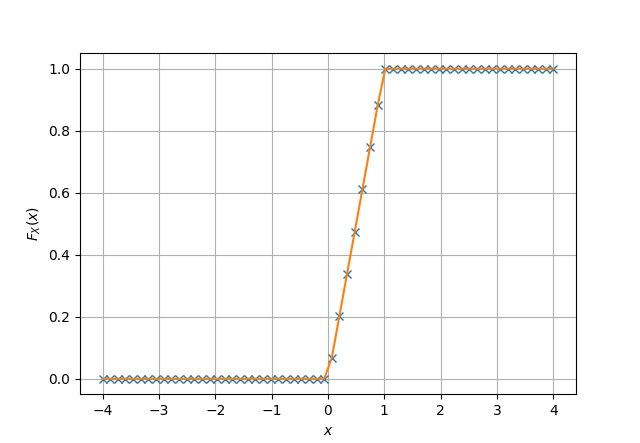
\includegraphics[width=\columnwidth]{./figs/cdf_plot.png}
		\caption{The CDF of $U$}
		\label{fig-1.2}
	\end{figure}
	
	\item Find a  theoretical expression for $F_{U}(x)$
	
	\solution The PDF of $U$ is given by
	\begin{align}
		p_{U}(x) = 
		\begin{cases}
			1 & x \in [0, 1] \\
			0 & \text{otherwise}
		\end{cases}
	\end{align}
	
	The CDF of $U$ is given by
	\begin{align}
		F_{U}(x) = \pr{U \le x} = \int_{-\infty}^x p_{U}(x) ~\mathrm{d}x
	\end{align}
	
	If $x<0$,
	\begin{align}
		\int_{-\infty}^x p_{U}(x) ~\mathrm{d}x = \int_{-\infty}^x 0 ~\mathrm{d}x = 0
	\end{align}
	
	If $x \in [0, 1]$,
	\begin{align}
		\int_{-\infty}^x p_{U}(x) ~\mathrm{d}x &= \int_{-\infty}^0 0 ~\mathrm{d}x + \int_0^x 1 ~\mathrm{d}x \\
		&= 0 + x \\
		&= x
	\end{align}
	
	If $x>1$,
	\begin{multline}
		\int_{-\infty}^x p_{U}(x) ~\mathrm{d}x \\= \int_{-\infty}^0 0 ~\mathrm{d}x + \int_0^1 1 ~\mathrm{d}x +  \int_1^x 0 ~\mathrm{d}x 
	\end{multline}
	\begin{align}
		\int_{-\infty}^x p_{U}(x) ~\mathrm{d}x &= 0 + 1 + 0 \\
		&= 1
	\end{align}
	
	Therefore, we obtain the CDF of $U$ as
	\begin{align}
		F_{U}(x) = 
		\begin{cases}
			0 & x < 0 \\
			x & 0 \le x \le 1 \\
			1 & x > 1
		\end{cases}
	\end{align}
	
	\item The mean of $U$ is defined as
	\begin{align}
		\mean{U} = \frac{1}{N}\sum_{i=1}^{N}U_i
	\end{align}
	and its variance as
	\begin{align}
		\var{U} = \mean{U- \mean{U}}^2 
	\end{align}
	Write a C program to  find the mean and variance of $U$
	
	\solution The c code for 1.4 can be obtained from
	\begin{lstlisting}
	wget https://github.com/karthik6281/AI1110-Assignments/blob/main/random_numbers/1/1_4.c
	wget https://github.com/karthik6281/AI1110-Assignments/blob/main/random_numbers/1/coeffs.h
	\end{lstlisting}
	Execute the following lines
	\begin{lstlisting}
		gcc 1_4.c -lm
		./a.out
	\end{lstlisting}
	\begin{align}
		\text{Mean} &= 0.500137 \\
		\text{Variance} &= 0.083251
	\end{align}
	
	\item Verify your result theoretically given that
	\begin{align}
		\mean{U^k} = \int_{-\infty}^{\infty}x^k \mathrm{d}F_{U}(x)
	\end{align}
		
	\solution 
		\begin{equation}
E\sbrak{U^k} = \int_{-\infty}^{\infty}x^kdF_{U}(x)
\end{equation}
\begin{align}
&dF_{U}(x)=dx\\
&\therefore E[U^k]=\int_{-\infty}^{\infty} x^k dx\\
&E[U]=\int_{0}^{1} x dx=\frac{1}{2}\\
&E[U^2]=\int_{0}^{1} x^2 dx=\frac{1}{3}\\
&\because P_{X}(x)=0 ,\forall x \in (1,\infty)\cap (-\infty,0)\\
&Var(X)=E[U^2]-(E[U])^2=\frac{1}{3}-\frac{1}{4}=\frac{1}{12}
\end{align}
	
	\section{Central Limit Theorem}

	\begin{enumerate}[label=\thesection.\arabic*,ref=\thesection.\theenumi]
	\item Generate $10^6$ samples of the random variable
	\begin{align}
		X = \sum_{i=1}^{12}U_i -6
	\end{align}

	using a C program, where $U_i, i = 1,2,\dots, 12$ are  a set of independent uniform random variables between 0 and 1 and save in a file called gau.dat
	
	\solution The c code for 2.1 can be obtained from
	\begin{lstlisting}
		wget https://github.com/karthik6281/AI1110-Assignments/blob/main/random_numbers/2/2_1.c
		wget https://github.com/karthik6281/AI1110-Assignments/blob/main/random_numbers/2/coeffs.h
	\end{lstlisting}
	Execute the following lines
	\begin{lstlisting}
		gcc 2_1.c -lm
		./a.out
	\end{lstlisting}
		
	\item Load gau.dat in Python and plot the empirical CDF of $X$ using the samples in gau.dat. What properties does a CDF have?

	\solution The python code for 2.2 can be obtained from
	\begin{lstlisting}
		wget https://github.com/karthik6281/AI1110-Assignments/blob/main/random_numbers/2/2_2.py
	\end{lstlisting}
	Execute the following lines
	\begin{lstlisting}
		python3 2_2.py
	\end{lstlisting}
	\begin{figure}
		\centering
		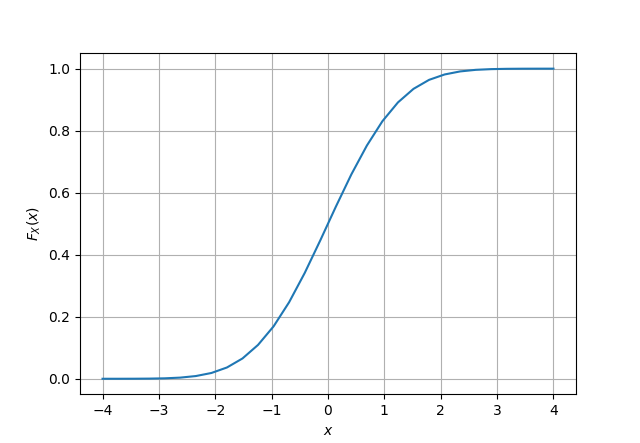
\includegraphics[width=\columnwidth]{./figs/2_2_fig.png}
		\caption{The CDF of $X$}
		\label{fig-2.2}
	\end{figure}
	
	\begin{itemize}
\item $\Phi(x)=P(Z \leq x)= \frac{1}{\sqrt{2 \pi}} \int_{-\infty}^{x}\exp\left\{-\frac{u^2}{2}\right\} du$
\item $\lim \limits_{x\rightarrow \infty} \Phi(x)=1, \hspace{5pt} \lim \limits_{x\rightarrow -\infty} \Phi(x)=0$
\item  $\Phi(0)=\frac{1}{2}$
\item  $\Phi(-x)=1-\Phi(x)$
\end{itemize}
	\item Load gau.dat in Python and plot the empirical PDF of $X$ using the samples in gau.dat. The PDF of $X$ is defined as
	\begin{align}
		p_{X}(x) = \frac{\der{}}{\der{x}}F_{X}(x)
	\end{align}
	What properties does the PDF have?
	
	\solution The python code for 2.3 can be obtained from
	\begin{lstlisting}
		wget https://github.com/karthik6281/AI1110-Assignments/blob/main/random_numbers/2/2_3.py
	\end{lstlisting}
	Execute the following lines
	\begin{lstlisting}
		python3 2.3.py
	\end{lstlisting}
	\begin{figure}
		\centering
		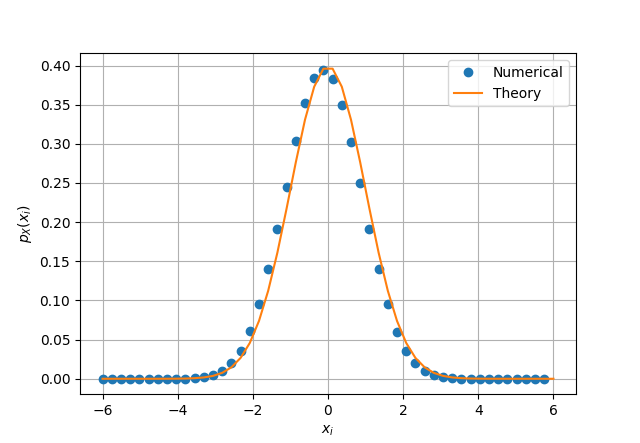
\includegraphics[width=\columnwidth]{./figs/2_3_fig.png}
		\caption{The PDF of $X$}
		\label{fig-2.3}
	\end{figure}
	
	Every PDF is bounded between $0$ and $1$ and
	\begin{align}
		\int_{-\infty}^{\infty} p_{X}(x) ~\mathrm{d}x = 1
	\end{align}
	
	In this case, the PDF is symmetric about $x = 0$ and graph is bell shaped
	
	\item Find the mean and variance of $X$ by writing a C program
	
	\solution the c code for 2.4 can be obtained from
	\begin{lstlisting}
		wget https://github.com/karthik6281/AI1110-Assignments/blob/main/random_numbers/2/2_4.c
		wget https://github.com/karthik6281/AI1110-Assignments/blob/main/random_numbers/2/coeffs.h
	\end{lstlisting}
	execute the following lines
	\begin{lstlisting}
		gcc 2_4.c -lm
		./a.out
	\end{lstlisting}
	\begin{align}
		\text{Mean} &= 0.000294 \\
		\text{Variance} &= 0.999561 
	\end{align}	
	
	\item Given that
	\begin{align}
		p_{X}(x) = \frac{1}{\sqrt{2\pi}}\exp\brak{-\frac{x^2}{2}}, -\infty < x < \infty,
	\end{align}
	repeat the above exercise theoretically
	
	\solution The mean of $X$ is given by
	\begin{align}
		\mean{X} &= \int_{-\infty}^{\infty} \frac{x}{\sqrt{2\pi}}\exp\brak{-\frac{x^2}{2}} \mathrm{d}x 
	\end{align}
	$\implies x e^{-\frac{-x^2}{2}} $
	\text{is a odd function}
	\begin{align}
		\therefore \mean{X} &= \int_{-\infty}^{\infty} g(x) \mathrm{d}x = 0
	\end{align}
	
	Now, 
	\begin{align}
		\mean{X^2} &= \int_{-\infty}^{\infty} \frac{x^2}{\sqrt{2\pi}}\exp\brak{-\frac{x^2}{2}} \mathrm{d}x \\
		&= 2 \int_{0}^{\infty} \frac{x^2}{\sqrt{2\pi}}\exp\brak{-\frac{x^2}{2}} \mathrm{d}x
	\end{align}
	$\implies \frac{x^2}{\sqrt{2\pi}}\exp\brak{-\frac{x^2}{2}}$ is an even function
	
	By integration by parts,
	\begin{align}
		\mean{X^2} = \sqrt{\frac{2}{\pi}}  \int_{0}^{\infty} x \cdot x \exp\brak{-\frac{x^2}{2}} \der{x} 
	\end{align}
	\begin{multline}
		= \sqrt{\frac{2}{\pi}} \brak{\left. x \int x \exp\brak{-\frac{x^2}{2}} \der{x}}\right|_0^{\infty} \\- \sqrt{\frac{2}{\pi}}  \int_{0}^{\infty} 1 \cdot \int x \exp\brak{-\frac{x^2}{2}} \der{x}
	\end{multline}
	
	Substitute $t = \frac{x^2}{2} \implies \der{t} = x\der{x}$
	\begin{align}
		\int x \exp\brak{-\frac{x^2}{2}} \der{x} &= \int \exp(-t) \der{t} \\
		&= - \exp(-t) \\
		&= - \exp\brak{-\frac{x^2}{2}}
	\end{align}
	
	\begin{align}
		&\int_0^{\infty} - \exp\brak{-\frac{x^2}{2}} \der{x} \\
		\xleftrightarrow{x = t\sqrt{2}} &\int_0^{\infty} -\exp(-t^2) \der{t}\sqrt{2} \\
		&= -{\sqrt{2}} \int_0^{\infty} \exp(-t^2) \der{t} \\
		&= - \sqrt{\frac{\pi}{2}}
	\end{align}
	
	Therefore,
	\begin{align}
		\mean{X^2} &= 0 - \sqrt{\frac{2}{\pi}} \brak{- \sqrt{\frac{\pi}{2}}} \\
		&= 1 \\
		\therefore \var{X} &= \mean{X^2} - \brak{\mean{X}}^2 \\
		&= 1 - 0 \\
		&= 1
	\end{align}
	\end{enumerate}
	
	\section{From Uniform to Other}
	\begin{enumerate}[label=\thesection.\arabic*,ref=\thesection.\theenumi]
	\item Generate samples of 
	\begin{align}
		V = -2\ln\brak{1-U}
	\end{align}
	and plot its CDF
	\end{enumerate}
	\solution The c code for 3.1 can be obtained from
	\begin{lstlisting}
		wget https://github.com/karthik6281/AI1110-Assignments/blob/main/random_numbers/3/3_1.c
	\end{lstlisting}
	Execute the following lines
	\begin{lstlisting}
		gcc 3.1.c -lm
		./a.out
	\end{lstlisting}
	The python code for cdf can be obtained from
	\begin{lstlisting}
		wget https://github.com/karthik6281/AI1110-Assignments/blob/main/random_numbers/3/3_1.py
	\end{lstlisting}
	execute the following lines
	\begin{lstlisting}
		python3 3_1.py
	\end{lstlisting}
	\begin{figure}
		\centering
		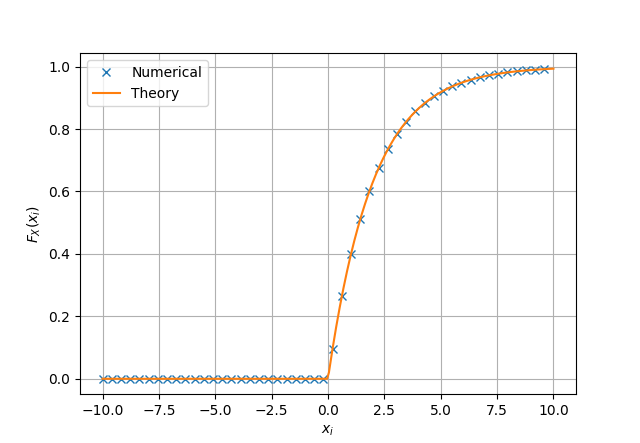
\includegraphics[width=\columnwidth]{./figs/3_1_cdf.png}
		\caption{The CDF of $V$}
		\label{fig-3.1}
	\end{figure}	
	
	\item Find a theoretical expression for $F_V(x)$
	
	\solution \begin{align}
 F_{V}(x)&=P(V \leq x)\\
 &=P(-2 ln(1-U) \leq x)\\
 &=P(1-e^{\frac{-x}{2}} \geq U)\\
 P(U<x)&=\int_{0}^{x} dx=x \hspace{10mm} \text{$0 < x < 1$}\\
 &\therefore P(1-e^{\frac{-x}{2}} \geq U)=1-e^{\frac{-x}{2}}, \forall x\geq 0 \\ 
 \nonumber
 \end{align}
	
	\section{Triangular Distribution}
	\begin{enumerate}[label=\thesection.\arabic*,ref=\thesection.\theenumi]
	\item Generate 
	\begin{align}
		T = U_1+U_2
	\end{align}
	\solution The c code for 4.1 can be obtained from
	\begin{lstlisting}
		wget https://github.com/karthik6281/AI1110-Assignments/blob/main/random_numbers/4/4_1.c
	\end{lstlisting}
	execute the following lines
	\begin{lstlisting}
		gcc 4_1.c -lm
		./a.out
	\end{lstlisting}
	
	\item Find the CDF of $T$
	
	\solution \begin{align}
    p_T(x) &= p_{U_1 + U_2}(x) = p_{U_1}(x) * p_{U_2}(x)\\
    p_T(x) &= \int_{-\infty}^{\infty}p_{U_1}(\tau)p_{U_2}(x - \tau)\\
    p_T(x) &= \int_0^1p_{U_2}(x - \tau)
\end{align}
\begin{align}
    \displaystyle p_T(x) = \begin{cases} 
    0 & \text{$x \leq 0$} \\  
    \int_0^x 1d\tau & \text{$0 < x < 1$} \\  
    \int_{x - 1}^1 1d\tau & \text{$1 \leq x < 2$} \\
    0 & \text{$x > 2$}
    \end{cases}
\end{align}
\begin{align}
    \displaystyle p_T(x) = \begin{cases} 
    0 & \text{$x \leq 0$} \\  
    x & \text{$0 < x < 1$} \\  
    2 - x & \text{$1 \leq x < 2$} \\
    0 & \text{$x > 2$}
    \end{cases}
\end{align}
Expression for CDF can be obtained by integrating $p_T(x)$ w.r.t. $X$
\begin{align}
    \displaystyle F_T(x) = \begin{cases} 
    0 & \text{$x \leq 0$} \\  
    \frac{x^2}{2} & \text{$0 < x < 1$} \\  
    -\frac{x^2}{2} + 2x - 1 & \text{$1 \leq x < 2$} \\
    1 & \text{$x > 2$}
    \end{cases}
\end{align}
	
	\item Find the PDF of $T$
	
	\solution The PDF of $T$ is given by
	\begin{align}
		p_T(t) &= \frac{d(F_{T}(t))}{dt} \\
		\therefore p_T(t) &=
		\begin{cases}
			0 & t < 0 \\
			t & 0 \le t \le 1 \\
			2 - t & 1 < t < 2 \\
			0 & t \ge 2
		\end{cases}
	\end{align}
	
	\item Find the theoretical expressions for the PDF and CDF of $T$
	
	\solution 
\begin{align}
P_{T}(t)=
\begin{cases}
0 & t<0\\
t & 0\leq t \leq 1\\
2-t  & 0< t \leq 2\\
0 & t>2 
\end{cases} 
\\   
F_{T}(t)=
\begin{cases}
0 & t<0\\
\frac{t^2}{2} & 0\leq t \leq 1\\
2t -\dfrac{t^2}{2} - 1  & 1< t \leq 2\\
1 & t>2
\end{cases}
\end{align}
	\item Verify your results through a plot
	
	\solution The codes that plots cdf and pdf can be obtained from
	\begin{lstlisting}
		wget https://github.com/karthik6281/AI1110-Assignments/blob/main/random_numbers/4/4_cdf.py
		wget https://github.com/karthik6281/AI1110-Assignments/blob/main/random_numbers/4/4_pdf.py
	\end{lstlisting}
	Execute the following lines
	\begin{lstlisting}
		python3 4_cdf.py
		python3 4_pdf.py
	\end{lstlisting}
	
	
	\end{enumerate}
	\end{enumerate}
	\begin{figure}
		\centering
		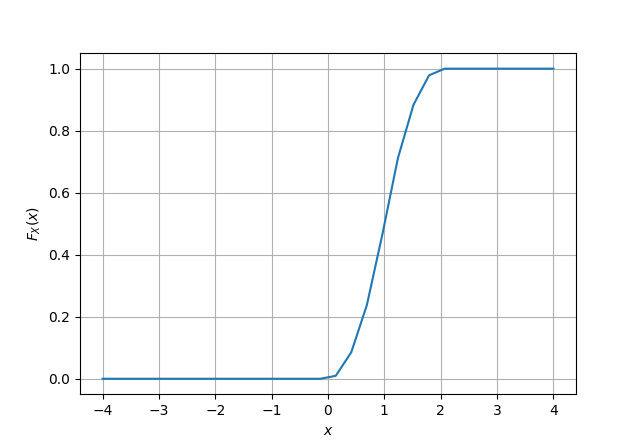
\includegraphics[width=\columnwidth]{./figs/4_cdf.png}
		\caption{The CDF of $T$}
	\end{figure}
	
	\begin{figure}
		\centering
		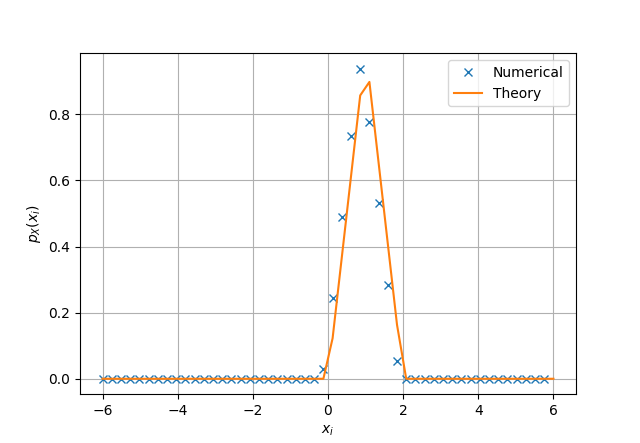
\includegraphics[width=\columnwidth]{./figs/4_pdf.png}
		\caption{The PDF of $T$}
	\end{figure}		
	
\section{Maximum Likelihood}
	\begin{enumerate}[label=\thesection.\arabic*,ref=\thesection.\theenumi]
	\item Generate equiprobable 	$X \in \cbrak{-1, 1}$
	
	\solution The c code for 5.1 can obtained from
	\begin{lstlisting}
		wget https://github.com/karthik6281/AI1110-Assignments/blob/main/random_numbers/5/5_1.c
		wget https://github.com/karthik6281/AI1110-Assignments/blob/main/random_numbers/5/coeffs.h
	\end{lstlisting}
	execute the following commands
	\begin{lstlisting}
	 gcc 5_1.c -lm
		./a.out
	\end{lstlisting}
	
	\item Generate 
	\begin{align}
		Y = AX+N
	\end{align}
	where $A = 5$ $~\mathrm{dB}$, $X \in \cbrak{-1, 1}$ is Bernoulli and $N \sim \gauss{0}{1}$
	
	\solution The c code for 5.2 can obtained from
	\begin{lstlisting}
		wget https://github.com/karthik6281/AI1110-Assignments/blob/main/random_numbers/5/5_2.c
		wget https://github.com/karthik6281/AI1110-Assignments/blob/main/random_numbers/5/coeffs.h
	\end{lstlisting}
	execute the following commands
	\begin{lstlisting}
	 gcc 5_2.c -lm
		./a.out
	\end{lstlisting}
	
	\item Plot $Y$
	
	\solution  Download the following Python code that plots Fig. \ref{fig-5.3}
	\begin{lstlisting}
		https://github.com/karthik6281/AI1110-Assignments/blob/main/random_numbers/5/5_3_plot.py
	\end{lstlisting}
	Run the code by executing
	\begin{lstlisting}
		python3 5_3_plot.py
	\end{lstlisting}
	\begin{figure}
		\centering
		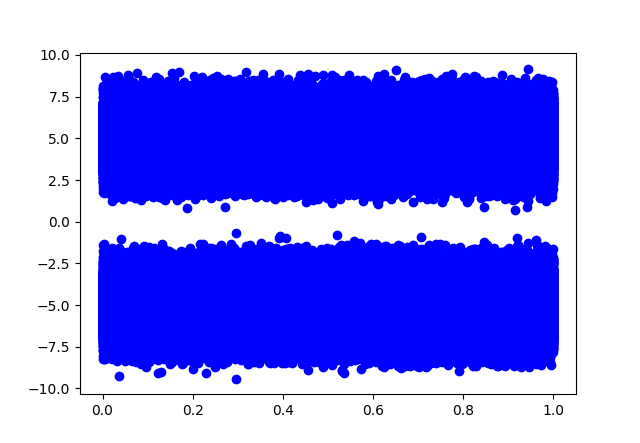
\includegraphics[width=\columnwidth]{./figs/5_3_plot.png}
		\caption{Plot of $Y$}
		\label{fig-5.3}
	\end{figure}
	
	\item Guess how to estimate $X$ from $Y$
	
	\solution
	\begin{align}
		X = 
		\begin{cases}
			1 & Y > 0 \\
			-1 & Y < 0
		\end{cases}
	\end{align}
	
	\item Find 
	\begin{align}
		P_{e|0} = \pr{\hat{X} = -1|X=1}
	\end{align}
	and 
	\begin{align}
		P_{e|1} = \pr{\hat{X} = 1|X=-1}
	\end{align}
	
	\solution 
	$\hat{X} = -1 \implies Y < 0$
	
	Given $X = +1$ , $Y < 0$ $\implies$ $5 + N < 0$ $\implies N < -5$
	\begin{align}
		\pr{\hat{X}=-1|X=1} &= \pr{N<-5} \\
		&= 1 - \pr{N>-5} \\
		&= 1 - Q(-5)	\\
		&= Q(5)
	\end{align}
	
	Similarly $\hat{X} = 1 \implies Y > 0$
	
	Given $X = -1$ , $Y > 0$ $\implies$ $-5 + N > 0$ $\implies N > 5$
	\begin{align}
		\pr{\hat{X}=1|X=-1} &= \pr{N>5} \\
		&= Q(5)		
	\end{align}
	
	\item Find $P_e$ assuming that $X$ has equiprobable symbols
	
	\solution 
	\begin{align}
		P_e = \pr{X=-1} P_{e|0} + \pr{X=1} P_{e|1}
	\end{align}
	From question, $\pr{X=-1} = \pr{X=1} = \frac12$
	\begin{align}
		P_e &= 2 \cdot (\frac12 Q(5) ) \\
		&= Q(5)	
	\end{align}		
	
	\item Verify by plotting the theoretical $P_e$ with respect to $A$ from $0$ to $10 ~\mathrm{dB}$
	
	\solution 
	$\hat{X} = 1 \implies Y > 0$
	
	then, $X = -1$ , $Y > 0$ $\implies$ $-A + N > 0$ $\implies N > A$
	\begin{align}
	P_{e|0} &= \pr{N>A} = Q(A)
   \end{align}

similarly ;
\begin{align}
	\pr{N < -A} = Q(A)
\end{align}
	
	The python code for 5.7 can be obtained from
	\begin{lstlisting}
		wget https://github.com/karthik6281/AI1110-Assignments/blob/main/random_numbers/5/5_7.py
	\end{lstlisting}
	Execute the following commands
	\begin{lstlisting}
		python3 5_7.py
	\end{lstlisting}
	\begin{figure}
		\centering
		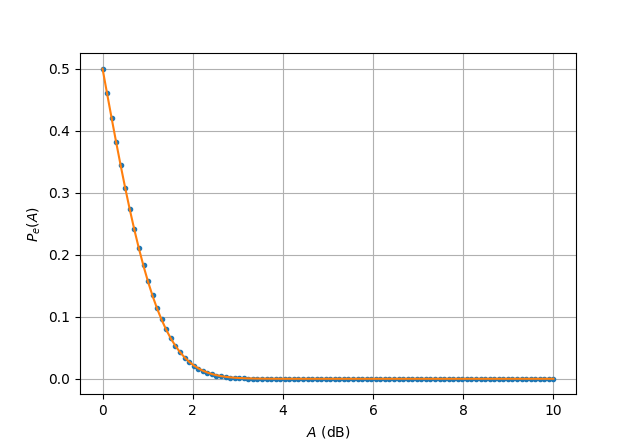
\includegraphics[width=\columnwidth]{./figs/5_7.png}
		\caption{Plot of $P_e$}
		\label{fig-5.7}
	\end{figure}
	
	\item Now, consider a threshold $\delta$  while estimating $X$ from $Y$. Find the value of $\delta$ that minimizes the theoretical $P_e$
	
	\solution 
	To estimate $X$ from $Y$, we now consider the following:
\begin{align}
    X = 
    \begin{cases}
        1, & Y > \delta \\
        -1, & Y < \delta
    \end{cases}
\end{align}
Therefore,
$\hat{X} = -1 \implies Y < \delta$
	
	then, $X = 1$ , $Y > 0$ $\implies$ $A + N < \delta$ $\implies N < \delta - A$
\begin{align}
P_{e|0} &= \pr{N < \delta - A} \\
&= \int _{-\infty} ^{\delta - A} \frac{1}{\sqrt{2\pi}} e^{-\frac{x^2}{2}} dx \\
&= \int _{A - \delta} ^{\infty} \frac{1}{\sqrt{2\pi}} e^{-\frac{x^2}{2}} dx \\
&= Q_N(A - \delta) 
\end{align}
Similarly
\begin{align}
P_{e|1} &= Q_N(A+\delta) 
\end{align}
\begin{align}
P_e &= \frac{1}{2}(Q_N(A - \delta) + Q_N(A + \delta)) 
\end{align}
To minimise $P_e$, we differentiate w.r.t $\delta$:
\begin{align}
0 &= \frac{d}{d\delta} \left(\frac{1}{2}(Q_N(A - \delta) + Q_N(A + \delta))\right) \\
&= \frac{1}{2} (\frac{1}{\sqrt{2\pi}} e^{-\frac{(\delta - A)^2}{2}} - \frac{1}{\sqrt{2\pi}} e^{-\frac{(A + \delta)^2}{2}} ) \\
\intertext{From which we obtain}
\implies \delta &= A = -A
\implies \delta = 0
\end{align}
	\item Repeat the above exercise when 
	\begin{align}
		p_{X}(-1) = p
	\end{align}
	
	\solution	
	\begin{align}
		P_e &= p_X(1) P_{e|0} + p_X(-1) P_{e|1} \\
		&= (1-p) Q(A-\delta) + p Q(A+\delta) 
	\end{align}
	
To minimise $P_e$, we differentiate w.r.t $\delta$:
\begin{align}
	0 &= p \frac{1}{\sqrt{2\pi}} e^{-\frac{(\delta - A)^2}{2}} - (1-p)\frac{1}{\sqrt{2\pi}} e^{-\frac{(A + \delta)^2}{2}} 
\end{align}
 Taking $\ln$ on both sides we have:
 \begin{align}
    \ln{p} - \frac{(\delta - A)^2}{2} &= \ln{1-p} + \frac{(\delta + A)^2}{2} \\
    \implies \delta &= \frac{1}{2A} \ln{\frac{1-p}{p}}
 \end{align}
	\item Repeat the above exercise using the MAP criterion	
	
	\solution Assume that $\pr{X = -1} = p$, and $\pr{X = 1} = (1-p)$. Then, using the Law of Total Probability,
we have:
\begin{align}
\nonumber p_Y(y) &= p_{Y|X = -1}(y|-1) \pr{X = -1} \\
&+ p_{Y| X = 1}(y|1) \pr{X = 1} \\
\nonumber &= p \times p_{(-A + N)}(y) \\
&+ (1-p) \times p_{(A+N)} (y) 
\end{align}
 
where $p_Y(y)$ is the pdf of $Y$. Now, $p_{(-A + N)}$ is just the pdf of a shifted
normal distribution, and therefore:
\begin{align}
    p_Y(y) &=  p \frac{e^{-\frac{(y+A)^2}{2}}}{\sqrt{2\pi}} + \left(1-p\right) \frac{e^{-\frac{(y-A)^2}{2}}}{\sqrt{2\pi}}
\end{align}
To use the MAP criterion, we must find $p_{X|Y}(x|y)$. To do this, we use the Theorem of Conditional Probability:
\begin{align}
    p_{X|Y}(x|y) &= \frac{p_{Y|X}(y|x) \times p_X(x)}{p_Y(y)}
\end{align}
When $X=1$, we have:
\begin{align}
    p_{X|Y}(1|y) &= \frac{p_{Y|X}(y|1) \times p_X(1)}{p_Y(y)} \\
    &= \frac{\left(1-p\right) \frac{e^{-\frac{(y-A)^2}{2}}}{\sqrt{2\pi}}}{ p \frac{e^{-\frac{(y+A)^2}{2}}}{\sqrt{2\pi}} + \left(1-p\right) \frac{e^{-\frac{(y-A)^2}{2}}}{\sqrt{2\pi}}} \\
    &= \frac{\left(1-p\right) e^{2yA}}{p + \left(1-p\right) e^{2yA}}
\end{align}
Similarly, when $X = -1$, we get:
\begin{align}
    p_{X|Y}(-1|y) &= \frac{p}{p + \left(1-p\right) e^{2yA}} 
\end{align}
Therefore, when $ p_{X|Y}(1|y) >  p_{X|Y}(-1|y)$, we have:
\begin{align}
    \frac{\left(1-p\right) e^{2yA}}{p + \left(1-p\right) e^{2yA}} &> \frac{p}{p + \left(1-p\right) e^{2yA}} \\
    e^{2yA} &> \frac{p}{\left(1-p\right)} \\
    \label{eq:y-condition}
    y &> \frac{1}{2A} \ln{\frac{p}{\left(1-p\right)}}
\end{align}
Therefore, when Eq. \eqref{eq:y-condition}, we can assert that $X = 1$, and $X = -1$ otherwise.
Now, consider when $p = \frac{1}{2} $.
We have:
\begin{align}
    y &> \frac{1}{2A} \ln{\frac{p}{\left(1-p\right)}} \\
    &= \frac{1}{2A} \ln{1} \\
    &= 0
\end{align}
Therefore, when $y > 0$, we choose $X = 1$, and we choose $X = -1$ otherwise.

	\end{enumerate}
	\section{Gaussian to Other}
	\begin{enumerate}[label=\thesection.\arabic*,ref=\thesection.\theenumi]
	\item Let $X_1 \sim  \gauss{0}{1}$ and $X_2 \sim  \gauss{0}{1}$. Plot the CDF and PDF of
	\begin{align}
		V = X_1^2 + X_2^2
	\end{align}
	
	\solution The c code to generate data can be obtained from
	\begin{lstlisting}
		wget https://github.com/karthik6281/AI1110-Assignments/blob/main/random_numbers/6/6_1.c
		wget https://github.com/karthik6281/AI1110-Assignments/blob/main/random_numbers/6/coeffs.h
	\end{lstlisting}
	Execute the following commands
	\begin{lstlisting}
		gcc 6_1.c -lm
		./a.out
	\end{lstlisting}
	
  The codes that plot cdf and pdf can be obtained from
	\begin{lstlisting}
		wget https://github.com/karthik6281/AI1110-Assignments/blob/main/random_numbers/6/6_1_cdf.c
		wget https://github.com/karthik6281/AI1110-Assignments/blob/main/random_numbers/6/6_1_pdf.c
		
	\end{lstlisting}
	Run the code by executing
	\begin{lstlisting}
		python3 6_!.cdf.py
		python3 6_1.pdf.py
	\end{lstlisting}
	\begin{figure}
		\centering
		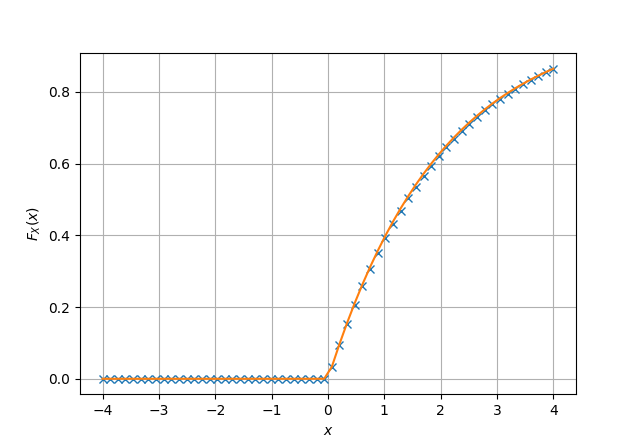
\includegraphics[width=\columnwidth]{./figs/6_1.cdf.png}
		\caption{CDF of $V$}
		\label{fig-6.1}
	\end{figure}
	\begin{figure}
		\centering
		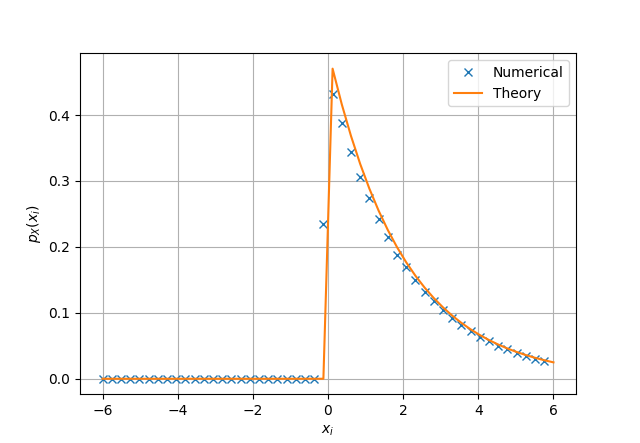
\includegraphics[width=\columnwidth]{./figs/6_1.pdf.png}
		\caption{PDF of $V$}
		\label{fig-6.2}
	\end{figure}
	
	\item If
	\begin{align}
		F_{V}(x) = 
		\begin{cases}
			1 - e^{-\alpha x} & x \geq 0 \\
			0 & x < 0,
		\end{cases}	
	\end{align}
	find $\alpha$
	
	\solution Let $R \ge 0, \Theta \in [0, 2\pi]$
	\begin{align}
		X_1 = R\cos\Theta  \\
		X_2 = R\sin\Theta 
	\end{align}
	such that $V = X_1^2 + X_2^2 = R^2$
	 
	 The Jacobian matrix transforming $R$, $\Theta$ to $X_1, X_2$  is defined as 
	 
	\begin{align}
		\vec{J} &= \myvec{
			\frac{\partial X_1}{\partial R} & \frac{\partial X_1}{\partial \Theta} \\
			\frac{\partial X_2}{\partial R} & \frac{\partial X_2}{\partial \Theta}
		} \\
		&= \myvec{
			\cos\Theta & -R\sin\Theta \\
			\sin\Theta & R\cos\Theta
		} \\
		\implies \mydet{\vec{J}} &= R\cos^2\Theta + R\sin^2\Theta = R
	\end{align}
	
	Then
		\begin{align}
		p_{R, \Theta} \brak{r, \theta} &= p_{X_1,X_2}\brak{x_1,x_2} \mydet{\vec{J}} \\
			&= \frac{R}{2\pi}\exp{\brak{-\frac{X_1^2 + X_2^2}{2}}} \\
			&= \frac{R}{2\pi}\exp{\brak{-\frac{R^2}{2}}}
			\label{eq:joint}
		\end{align}
we can find,
		\begin{align}
			p_R(r) &= \int_{0}^{2\pi}p_{R, \Theta}(r, \theta)d\theta \\
			&= R\exp{\brak{-\frac{R^2}{2}}}
		\end{align}
		
	We can find cdf by
	\begin{align}
		F_R(r) &= \pr{R \le r} \\
		&= \int_0^r p_R(r) \der{r} \\
		&= \int_0^r r \exp\brak{-\frac{r^2}{2}} \der{r} \\
		&= - \left. \exp\brak{-\frac{r^2}{2}} \right|_0^r \\
		&= 1 - \exp\brak{-\frac{r^2}{2}} \quad \text{for } r \ge 0
	\end{align}		
	
	But we need to find $ F_V(x) $ which can be wriiten as
	\begin{align}
		F_V(x) &= F_R(\sqrt{x}) \\
		&= 1 - \exp\brak{-\frac{x}{2}} \quad \text{for } x \ge 0
	\end{align}
	
	And the PDF of $V$ is given by
	\begin{align}
		p_V(x) &= \frac{\der{}}{\der{x}} F_V(x) \\
		&= \frac12 \exp\brak{-\frac{x}{2}} 
	\end{align}
	
	Therefore,
	\begin{align}
		F_V(x) &= 
		\begin{cases}
			1 - \exp\brak{-\dfrac{x}{2}} & x \geq 0 \\
			0 & \text{otherwise}
		\end{cases}	\\
		p_V(x) &= 
		\begin{cases}
			\dfrac12 \exp\brak{-\dfrac{x}{2}} & x \geq 0 \\
			0 & \text{otherwise}
		\end{cases}
	\end{align}
	\begin{align}
		\therefore \alpha = \frac12
	\end{align}
	
	\item Plot the CDF and PDF of
	\begin{align}
		A = \sqrt{V}
	\end{align}
	
	\solution The c code to generate 
	\begin{lstlisting}
		wget https://github.com/karthik6281/AI1110-Assignments/blob/main/random_numbers/6/6_3.c
	\end{lstlisting}
	executing the following
	\begin{lstlisting}
		gcc 6_3.c -lm
		./a.out
	\end{lstlisting}
	
	The codes for cdf and pdf can be obtained from
	\begin{lstlisting}
	wget https://github.com/karthik6281/AI1110-Assignments/blob/main/random_numbers/6/6_3_cdf.py
	wget https://github.com/karthik6281/AI1110-Assignments/blob/main/random_numbers/6/6_3_cdf.py
	
	\end{lstlisting}
	execute the following
	\begin{lstlisting}
		python3 6_3_cdf.py
		python3 6_3_pdf.py
	\end{lstlisting}
	\begin{figure}
		\centering
		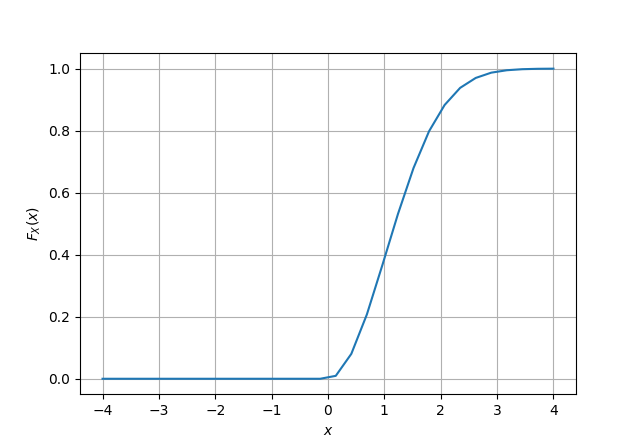
\includegraphics[width=\columnwidth]{./figs/6_3_cdf.png}
		\caption{CDF of $A$}
		\label{fig-6.3}
	\end{figure}
	\begin{figure}
		\centering
		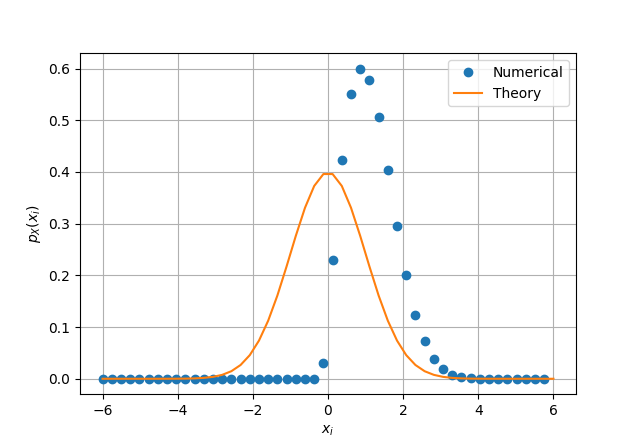
\includegraphics[width=\columnwidth]{./figs/6_3_pdf.png}
		\caption{PDF of $A$}
		\label{fig-6.4}
	\end{figure}
	
	The CDF of $A$ for $x > 0$:
	\begin{align}
		F_A(x) &=  F_V(x^2) \\
		&= 1 - \exp\brak{-\frac{x^2}{2}}
	\end{align}
	
	Pdf of $A$ for $x > 0$:
	\begin{align}
		p_A(x) &= \frac{\der{}}{\der{x}} F_A(x) \\
		&= x \exp\brak{-\frac{x^2}{2}}
	\end{align}
	
	Therefore,
	\begin{align}
		F_A(x) &= 
		\begin{cases}
			1 - \exp\brak{-\dfrac{x^2}{2}} & x \geq 0 \\
			0 & \text{otherwise}
		\end{cases}	\\
		p_A(x) &= 
		\begin{cases}
			x \exp\brak{-\dfrac{x^2}{2}} & x \geq 0 \\
			0 & \text{otherwise}
		\end{cases}
	\end{align}
	
	\end{enumerate}
\end{document}
